% replace all text with your own text.
% in this template few examples are mention
\chapter{Methodology}
\label{ch:method} % Label for method chapter

\section{Importing the necessary libraries}

Importing the required Python libraries used for machine learning tasks and training models is the first step in any data processing task. These libraries facilitate various functionalities like visualization process, data manipulation, data modification, statistical analysis, training and testing of various deep learning models, and other machine learning tasks. Python has various external and built-in libraries that can be imported into the Jupyter Notebook. The libraries used for credit card fraud detection systems are as follows -

\subsection{Pandas}
Pandas is a powerful Python package made for analysis and data manipulation. It makes structured data processing simple by offering data structures like DataFrames. Pandas make it easy to effectively carry out operations like data cleansing, modification, data aggregation, data visualization, and data exploration.

\subsection{Numpy}
Numpy is a free Python software package that is intended for numerical operations on data in the form of arrays and multi-dimensional arrays. It provides standard mathematical techniques for data manipulation using linear algebra and gives users a variety of tools to manage such arrays and perform statistical operations. Basic array operations made possible by NumPy include indexing, slicing, adding, multiplying, and reshaping arrays.

\subsection{Matplotlib}
Matplotlib is a  Python data visualization package that offers a wide range of data visualization tools and functions that make data reading easy. A variety of graph types, including scatterplots, pie charts, bars, and histograms are available. Furthermore, these graphs may be exported in JPEG or PNG formats

\subsection{Seaborn}
Seaborn is one the best data visualization libraries used in Python and is a higher version of Matplotlib. It facilitates various functions and methods that can operate in data frames to perform the statistical plotting of graphs like heatmaps and histograms. Various graphs provided by this library include bar charts, histograms, error charts, scatterplots, and also heat maps which are not available in Matplotlib. It also has a feature that can select the colors that can disclose the underlying patterns and trends in the data.

\subsection{Scikit-learn}
This Python library is available as open-source and is used to build various machine learning methods. To train different machine learning methods and deep learning models, such as decision trees, support vector machines (SVM), naive Bayes, and classifiers, It also provides a variety of classification, regression, clustering, supervised and unsupervised techniques. By determining the accuracy score and producing the classification report, it also aids in evaluating the trained model's correctness; nevertheless, it cannot execute neural network models.

\subsection{Xgboost}
XGBoost, also referred to as Extreme Gradient Boost is a powerful Python module in which regression and classification are commonly used tasks. Gradient boosting methods are used by XGBoost, which is well-known for its efficiency, scalability, and operational strength. To correct mistakes produced by earlier models, these algorithms successively train inadequate learners, which are usually decision trees. Performance and utilization of resources are optimized by the library through the use of distributed and concurrent computing techniques.

\section{Data Collection}
The dataset for the credit card fraud detection system is taken from an online source Kaggle. It contains details of transactions made by the credit card by the card holders that happened in 2 days. The data set consists of 31 columns which contain the results of the transformation by PCA as numerical data input. Namely V1, V2, V3….V28 are the primary components identified by PCA. Only 2 columns which are ‘Time’ and ‘Amount’ have not undergone PCA transformation. The ‘Time’ column contains the seconds passed between each transaction and the dataset’s initial transaction. The column name ‘Amount’ contains the transaction amount which may be utilized for cost-sensitive learning based on examples. The ‘Class’ column is the answer variable and has the response as 1 in the event of fraud and 0 if no fraud is identified. It is advisable to use the Area Under the Precision-Recall Curve (AUPRC) to measure the accuracy for class imbalance ratio whereas for imbalance class, accuracy by confusion matrix is meaningless.
.
\section{Reading the Dataset}
Reading the Dataset is the next step after collecting the data set which is used to analyze the fraud in online transactions through credit cards. It is crucial to read the dataset after importing the required libraries to comprehend the data that has been provided. This makes it easier to train, analyze, and visualize the model of the dataset. The dataset is read by loading the CSV file into a Pandas data frame using the pd.read\_csv() function. This may be accomplished by giving the user the complete path to the CSV file or just the path to the directory in the Python environment where the dataset is uploaded. Once the dataset has been imported, data exploration is carried out. To provide an overview of the data, the top few columns and their contents are shown using the df.head() method. Here, df.head(5) provides the details of the top 5 rows and columns 



\section{Data Analysis}
The following step after reading the data set is to examine the substance of the data by analyzing it once the dataset has been loaded and processed in the Notebook. It entails cleansing the data by eliminating irrelevant or undesired information and handling outliers and missing numbers. After the data has been imported and cleaned, data analysis is completed. This involves examining, sanitizing, and altering the data to extract valuable insights, draw conclusions, and facilitate decision-making. Gaining understanding, making forecasts, or just working towards a particular problem's solution are all aided by data analysis. 

Here, df.info() is used to get the information of the data frame which includes the data index, column name, non-null values, and the data type of that attribute. Then df.shape() is used to return the size or dimension of the data frame which is represented as the number of rows and columns. The result shows that the shape of the data frame is (284,807, 31) which denotes 284,807 rows and 31 columns. Similarly, df.describe() describes the data present in the data frame which helps to calculate statistical values like mean, median, etc. of the numerical values present in the provided data frame.


\section{Data Processing}
While processing the data set, the raw, unstructured data set is transformed into a clear, understandable form. Data pre-processing the the process of changing the data into relevant and appropriate forms before sending the data for training and testing. In this way, if the raw data contains any outliers, noise, missing values, or any irrelevant information, it can be removed before passing the data as input for the model which is the final data set. There are several  categories into which data preparation techniques are divided. Detecting outliers and addressing missing numbers are the two primary tasks of this phase. Various cleaning procedures are done to clean the data set by addressing problems which include noisy data, missing values, finding and removing outliers, and solving the differences. If users believe that the data is polluted, they are less inclined to trust data mining results. Values for a characteristic that differs from other data by more than two standard deviations might be classified as outliers. 

The process of data visualization is crucial to data analysis and investigation. The data visualization is supported by several built-in libraries in Python. This method presents the data in a highly graphical manner that facilitates better visual comprehension of the information, making it simpler to analyze trends and recognize patterns and correlations between several variables. Several graphs may be drawn, and each kind of graph depicts the data uniquely. The two Python libraries that are most frequently utilized when importing the graphical representation are Matplotlib and Seaborn. Many graph formats, including line, scatter, bar, and histogram plots, are supported by Matplotlib. However, Seaborn is based on Matplotlib and is an improved version of it. 

Checking for any missing values is done using the df.isna() function. Then, the data is processed for any duplicate values if present using the df.duplicates(). The result shows that there are 1081 duplicate values present in the dataset. These duplicate values are removed or dropped using the df.drop() function.

The given dataset contains the time and date of the transaction which can be used to determine the cases of fraud and valid transactions. The given data is plotted in a pie graph to visually represent the percentage of valid or legitimate transactions made with the credit card which is denoted as ‘0’ while the percentage of fraud transactions is denoted as ‘1’. The green part of the pie chart shows that ‘0’ i.e. the percentage of cases of legitimate transactions is 99.83\% while the red part of the pie chart displays the percentage of cases of fraud transactions which is 0.17\%. This data can simplify the process of identifying fraudulent transactions which helps financial institutions, and credit card owners from any fraudulent activities and transactions.


 \section{Training and Test Split}
 After the data processing of the given dataset which includes cleaning and visualizing the data, the next step is to divide the data set into training and testing data which is used to train the deep learning model. Dividing the data set into training and testing data ensures that the model can be trained on the training part of the data and then the model can be evaluated on the testing part of the data. This can be done by using the Scikit-learn library and the data is split in such a manner that around 80\% of the data is used for the training part i.e.\textbf{ x\_train }\& \textbf{y\_train }while the remaining 20\% of the data is used for the testing i.e. \textbf{x\_test }\&\textbf{ y\_test} and evaluation part. This ensures that the data is appropriately distributed for the model to learn effectively and generate accurate predictions. Also, splitting the dataset helps to avoid overfitting issues in which the model can strongly perform on training data but poorly on new data ensuring the establishment of a robust credit card fraud detection system that works effectively in the real world.

 



\section{Implementation}
\subsection{Logistic Regression}
 We Implement binary classification using Python's scikit-learn library. First, we split the dataset into training and testing sets. The training set is used to train the model, while the testing set is kept aside for evaluation. After training, the model predicts the labels for the test set. We then evaluate the model's performance using metrics like accuracy and F1 score, which consider the correctness of predictions. The confusion matrix provides a visual representation of the model's performance, helping us understand how well it's classifying instances. By analyzing these metrics and the confusion matrix, we gain insights into the model's effectiveness in correctly classifying instances into their respective classes


\section{Plot of the Dataset}


\begin{figure}[ht]
    \centering
    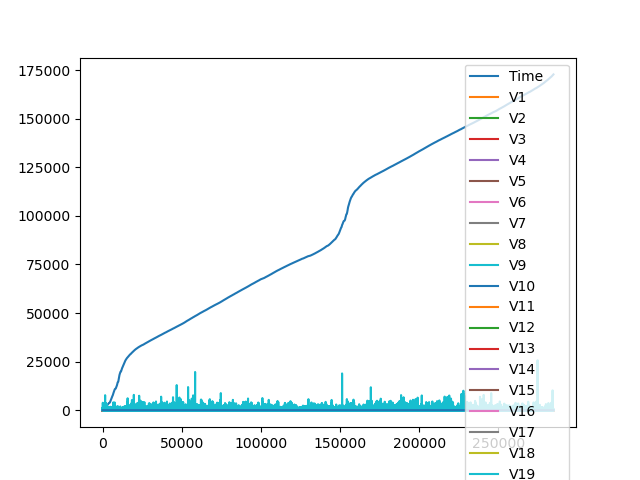
\includegraphics[scale=0.3]{figures/BasicPlot.png}
    \caption{Figure of the Data}
    \label{fig:Plot of the Data}
\end{figure}
\

\section{Table of the Dataset]}
\begin{table}[ht!]
    \centering
    \caption{Undergraduate report template structure}
    \label{tab:gen_template}
    \begin{tabular}{llll}     
        \toprule
        \multirow{7}{3cm}{Frontmatter} 
        & & Title Page & \\                  
        & & Abstract &    \\          
        & & Acknowledgements & \\                            
        & & Table of Contents &    \\                                
        & & List of Figures   &    \\                        
        & & List of Tables    &    \\                
        & & List of Abbreviations  &    \\                     
        & &   &    \\                        
        \multirow{7}{3cm}{Main text}
        & Chapter 1 & Introduction   &    \\                         
        & Chapter 2 & Literature Review   &    \\
        & Chapter 3 & Methodology   &    \\
        & Chapter 4 & Results    &    \\
        & Chapter 5 & Discussion and Analysis  &    \\
        & Chapter 6 & Conclusions and Future Work  &    \\        
        & Chapter 7 & Refection  &    \\          
        & &   &    \\                       
        \multirow{2}{3cm}{End matter}
        & & References  &    \\   
        & & Appendices (Optional)  &    \\ 
        & & Index (Optional)  &    \\ 
        \bottomrule
    \end{tabular}
\end{table}

\subsection{Example of a software/Web development main text structure}
\label{subsec:se_chpters}
Notice that the ``methodology'' Chapter of Software/Web development in Table~\ref{tab:soft_eng_temp} takes a standard software engineering paradigm (approach). Alternatively, these suggested sections can be the chapters of their own. Also, notice that ``Chapter 5'' in Table~\ref{tab:soft_eng_temp} is ``Testing and Validation'' which is different from the general report template mentioned in Table~\ref{tab:gen_template}. Check with your supervisor if in doubt.
\begin{table}[ht!]
    \centering
    \caption{Example of a software engineering-type report structure}
    \label{tab:soft_eng_temp}
    \begin{tabular}{lll}     
        \toprule                   
        Chapter 1 & Introduction   &    \\        
        Chapter 2 & Literature Review  &    \\                   
        Chapter 3 & Methodology   &    \\
        &               & Requirements specifications   \\
        &               & Analysis   \\
        &               & Design   \\
        &               & Implementations   \\
        Chapter 4 & Testing and Validation  &    \\
        Chapter 5 & Results and Discussion      &    \\
        Chapter 6 & Conclusions and Future Work  &    \\        
        Chapter 7 & Reflection  &    \\                          
        \bottomrule
    \end{tabular}
\end{table}

\subsection{Example of an algorithm analysis main text structure}
Some project might involve the implementation of a state-of-the-art algorithm and its performance analysis and comparison with other algorithms. In that case, the suggestion in Table~\ref{tab:algo_temp} may suit you the best. 
\begin{table}[ht!]
    \centering
    \caption{Example of an algorithm analysis type report structure}
    \label{tab:algo_temp}
    \begin{tabular}{lll}     
        \toprule                   
        Chapter 1 & Introduction  &    \\        
        Chapter 2 & Literature Review  &    \\                
        Chapter 3 & Methodology   &    \\
        &               & Algorithms descriptions  \\
        &               & Implementations   \\
        &               & Experiments design   \\
        Chapter 4 & Results       &  \\
        Chapter 5 & Discussion and Analysis  &    \\
        Chapter 6 & Conclusion and Future Work  &    \\        
        Chapter 7 & Reflection  &    \\          
        \bottomrule
    \end{tabular}
\end{table}

\subsection{Example of an application type main text structure}
If you are applying some algorithms/tools/technologies on some problems/datasets/etc., you may use the methodology section prescribed in Table~\ref{tab:app_temp}.  
\begin{table}[ht!]
    \centering
    \caption{Example of an application type report structure}
    \label{tab:app_temp}
    \begin{tabular}{lll}     
        \toprule                   
        Chapter 1 & Introduction  &    \\        
        Chapter 2 & Literature Review  &    \\                
        Chapter 3 & Methodology   &    \\
        &               & Problems (tasks) descriptions  \\
        &               & Algorithms/tools/technologies/etc. descriptions  \\        
        &               & Implementations   \\
        &               & Experiments design and setup   \\
        Chapter 4 & Results       &  \\
        Chapter 5 & Discussion and Analysis  &    \\
        Chapter 6 & Conclusion and Future Work  &    \\        
        Chapter 7 & Reflection  &    \\          
        \bottomrule
    \end{tabular}
\end{table}

\subsection{Example of a science lab-type main text structure}
If you are doing a science lab experiment type of project, you may use the  methodology section suggested in Table~\ref{tab:lab_temp}. In this kind of project, you may refer to the ``Methodology'' section as ``Materials and Methods.''
\begin{table}[ht!]
    \centering
    \caption{Example of a science lab experiment-type report structure}
    \label{tab:lab_temp}
    \begin{tabular}{lll}     
        \toprule                   
        Chapter 1 & Introduction  &    \\        
        Chapter 2 & Literature Review  &    \\                
        Chapter 3 & Materials and Methods   &    \\
        &               & Problems (tasks) description  \\
        &               & Materials \\        
        &               & Procedures  \\                
        &               & Implementations   \\
        &               & Experiment set-up   \\
        Chapter 4 & Results       &  \\
        Chapter 5 & Discussion and Analysis  &    \\
        Chapter 6 & Conclusion and Future Work  &    \\        
        Chapter 7 & Reflection  &    \\          
        \bottomrule
    \end{tabular}
\end{table}

\section{Example of an Equation in \LaTeX}
Eq.~\ref{eq:eq_example} [note that this is an example of an equation's in-text citation] is an example of an equation in \LaTeX. In Eq.~\eqref{eq:eq_example}, $ s $ is the mean of elements $ x_i \in \mathbf{x} $: 

\begin{equation}
\label{eq:eq_example} % label used to refer the eq in text
s = \frac{1}{N} \sum_{i = 1}^{N} x_i. 
\end{equation}

Have you noticed that all the variables of the equation are defined using the \textbf{in-text} maths command \$.\$, and Eq.~\eqref{eq:eq_example} is treated as a part of the sentence with proper punctuation? Always treat an equation or expression as a part of the sentence. 

\section{Example of a Figure in \LaTeX}
Figure~\ref{fig:chart_a} is an example of a figure in \LaTeX. For more details, check the link:

\href{https://en.wikibooks.org/wiki/LaTeX/Floats,_Figures_and_Captions}{wikibooks.org/wiki/LaTeX/Floats,\_Figures\_and\_Captions}.

\noindent
Keep your artwork (graphics, figures, illustrations) clean and readable. At least 300dpi is a good resolution of a PNG format artwork. However, an SVG format artwork saved as a PDF will produce the best quality graphics. There are numerous tools out there that can produce vector graphics and let you save that as an SVG file and/or as a PDF file. One example of such a tool is the ``Flow algorithm software''. Here is the link for that: \href{http://www.flowgorithm.org/download/}{flowgorithm.org}.
\begin{figure}[ht]
    \centering
    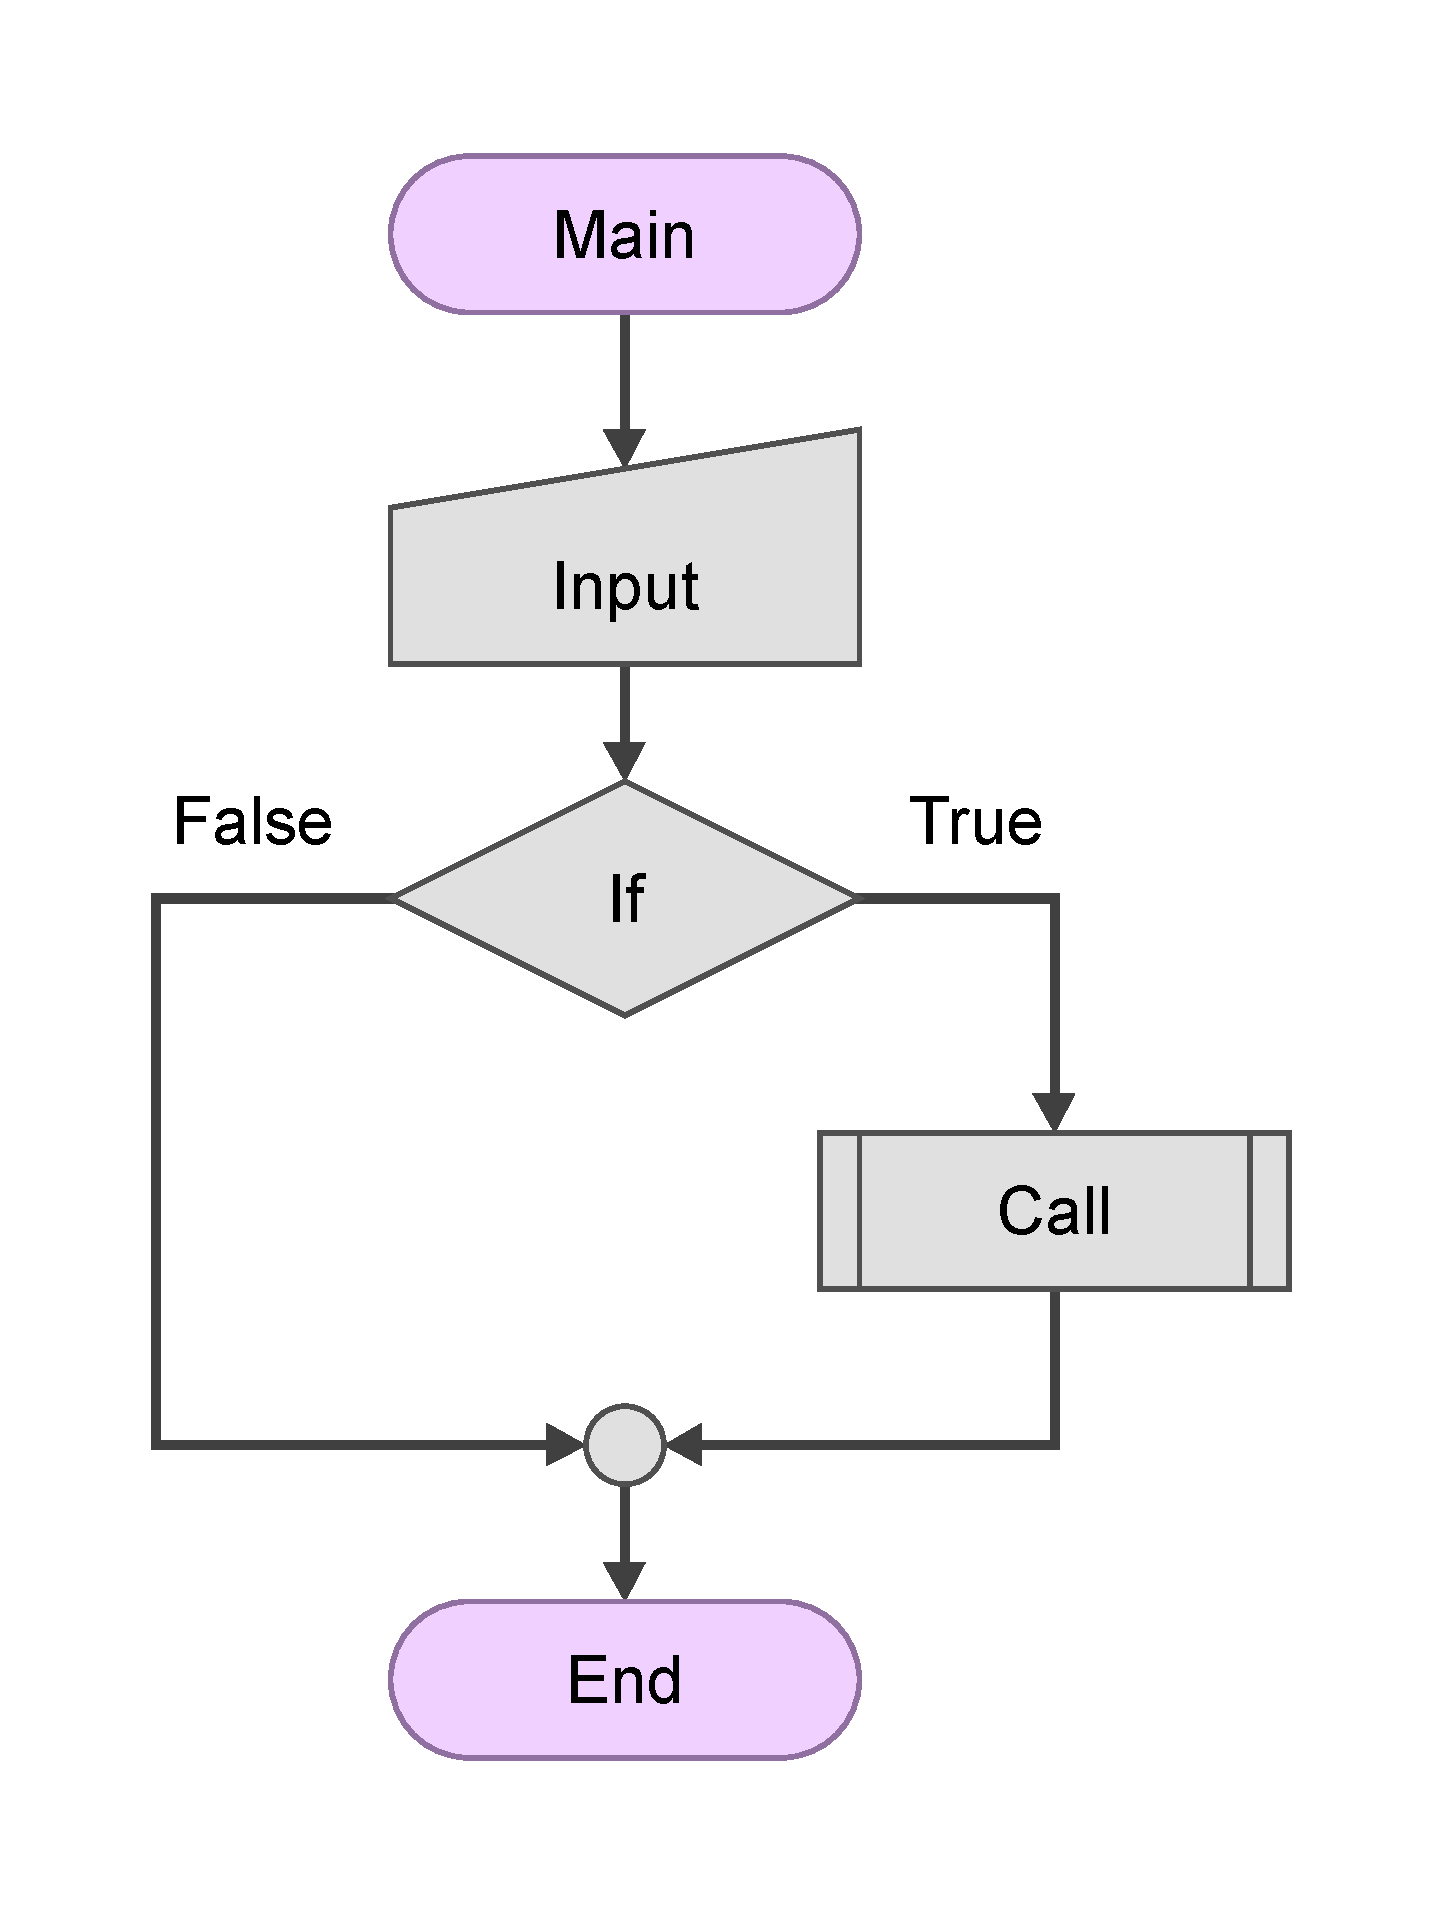
\includegraphics[scale=0.3]{figures/chart.pdf}
    \caption{Example figure in \LaTeX.}
    \label{fig:chart_a}
\end{figure}

\clearpage %  use command \clearpage when you want section or text to appear in the next page.

\section{Example of an algorithm in \LaTeX}
Algorithm~\ref{algo:algo_example} is a good example of an algorithm in \LaTeX.  
\begin{algorithm}
    \caption{Example caption: sum of all even numbers}
    \label{algo:algo_example}
    \begin{algorithmic}[1]
        \Require{$ \mathbf{x}  = x_1, x_2, \ldots, x_N$}
        \Ensure{$EvenSum$ (Sum of even numbers in $ \mathbf{x} $)}
        \Statex
        \Function{EvenSummation}{$\mathbf{x}$}
        \State {$EvenSum$ $\gets$ {$0$}}
        \State {$N$ $\gets$ {$length(\mathbf{x})$}}
        \For{$i \gets 1$ to $N$}                    
        \If{$ x_i\mod 2 == 0$}  \Comment check if a number is even?
        \State {$EvenSum$ $\gets$ {$EvenSum + x_i$}}
        \EndIf
        \EndFor
        \State \Return {$EvenSum$}
        \EndFunction
    \end{algorithmic}
\end{algorithm}
 
\section{Example of code snippet  in \LaTeX}

Code Listing~\ref{list:python_code_ex} is a good example of including a code snippet in a report. While using code snippets, take care of the following:
\begin{itemize}
    \item do not paste your entire code (implementation) or everything you have coded. Add code snippets only. 
    \item The algorithm shown in Algorithm~\ref{algo:algo_example} is usually preferred over code snippets in a technical/scientific report. 
    \item Make sure the entire code snippet or algorithm stays on a single page and does not overflow to another page(s).  
\end{itemize}

Here are three examples of code snippets for three different languages (Python, Java, and CPP) illustrated in Listings~\ref{list:python_code_ex}, \ref{list:java_code_ex}, and \ref{list:cpp_code_ex} respectively.  

\begin{lstlisting}[language=Python, caption={Code snippet in \LaTeX ~and  this is a Python code example}, label=list:python_code_ex]
import numpy as np

x  = [0, 1, 2, 3, 4, 5] # assign values to an array
evenSum = evenSummation(x) # call a function

def evenSummation(x):
    evenSum = 0
    n = len(x)
    for i in range(n):
        if np.mod(x[i],2) == 0: # check if a number is even?
            evenSum = evenSum + x[i]
    return evenSum
\end{lstlisting}

Here we used  the ``\textbackslash clearpage'' command and forced-out the second listing example onto the next page. 
\clearpage  %
\begin{lstlisting}[language=Java, caption={Code snippet in \LaTeX ~and  this is a Java code example}, label=list:java_code_ex]
public class EvenSum{ 
    public static int evenSummation(int[] x){
        int evenSum = 0;
        int n = x.length;
        for(int i = 0; i < n; i++){
            if(x[i]%2 == 0){ // check if a number is even?
                evenSum = evenSum + x[i];
            }
        }
        return evenSum;     
    }
    public static void main(String[] args){ 
        int[] x  = {0, 1, 2, 3, 4, 5}; // assign values to an array
        int evenSum = evenSummation(x);
        System.out.println(evenSum);
    } 
} 
\end{lstlisting}


\begin{lstlisting}[language=C, caption={Code snippet in \LaTeX ~and  this is a C/C++ code example}, label=list:cpp_code_ex]
int evenSummation(int x[]){
    int evenSum = 0;
    int n = sizeof(x);
    for(int i = 0; i < n; i++){
        if(x[i]%2 == 0){ // check if a number is even?
            evenSum = evenSum + x[i];
    	}
    }
    return evenSum;     
}

int main(){
    int x[]  = {0, 1, 2, 3, 4, 5}; // assign values to an array
    int evenSum = evenSummation(x);
    cout<<evenSum;
    return 0;
}
\end{lstlisting}



\section{Example of in-text citation style}
\subsection{Example of the equations and illustrations placement and reference in the text}
Make sure whenever you refer to the equations, tables, figures, algorithms,  and listings for the first time, they also appear (placed) somewhere on the same page or in the following page(s). Always make sure to refer to the equations, tables and figures used in the report. Do not leave them without an \textbf{in-text citation}. You can refer to equations, tables and figures more them once.

\subsection{Example of the equations and illustrations style}
Write \textbf{Eq.} with an uppercase ``Eq`` for an equation before using an equation number with (\textbackslash eqref\{.\}). Use ``Table'' to refer to a table, ``Figure'' to refer to a figure, ``Algorithm'' to refer to an algorithm and ``Listing'' to refer to listings (code snippets). Note that, we do not use the articles ``a,'' ``an,'' and ``the'' before the words Eq., Figure, Table, and Listing, but you may use an article for referring the words figure, table, etc. in general.

For example, the sentence ``A report structure is shown in \textbf{the} Table~\ref{tab:gen_template}'' should be written as ``A report structure is shown \textbf{in} Table~\ref{tab:gen_template}.'' 
 

\section{Summary}
Write a summary of this chapter.

~\\[5em]
\noindent
{\huge\textbf{Note:}} In the case of \textbf{software engineering} project a Chapter ``\textbf{Testing and Validation}'' should precede the ``Results'' chapter. See Section~\ref{subsec:se_chpters} for report organization of such project. 

